\documentclass{article}

\usepackage{graphicx}
\usepackage{tikz}
\usepackage{tikzsymbols}
\usetikzlibrary{calc,patterns,shapes.geometric}
\pagestyle{empty}
\usepackage[margin=0pt]{geometry}
\geometry{papersize={14in,12in}}

\def\centerarc[#1](#2)(#3:#4:#5){\draw[#1] ($(#2)+({#5*cos(#3)},{#5*sin(#3)})$) arc (#3:#4:#5);}

\begin{document}
	\begin{figure}
		\centering
		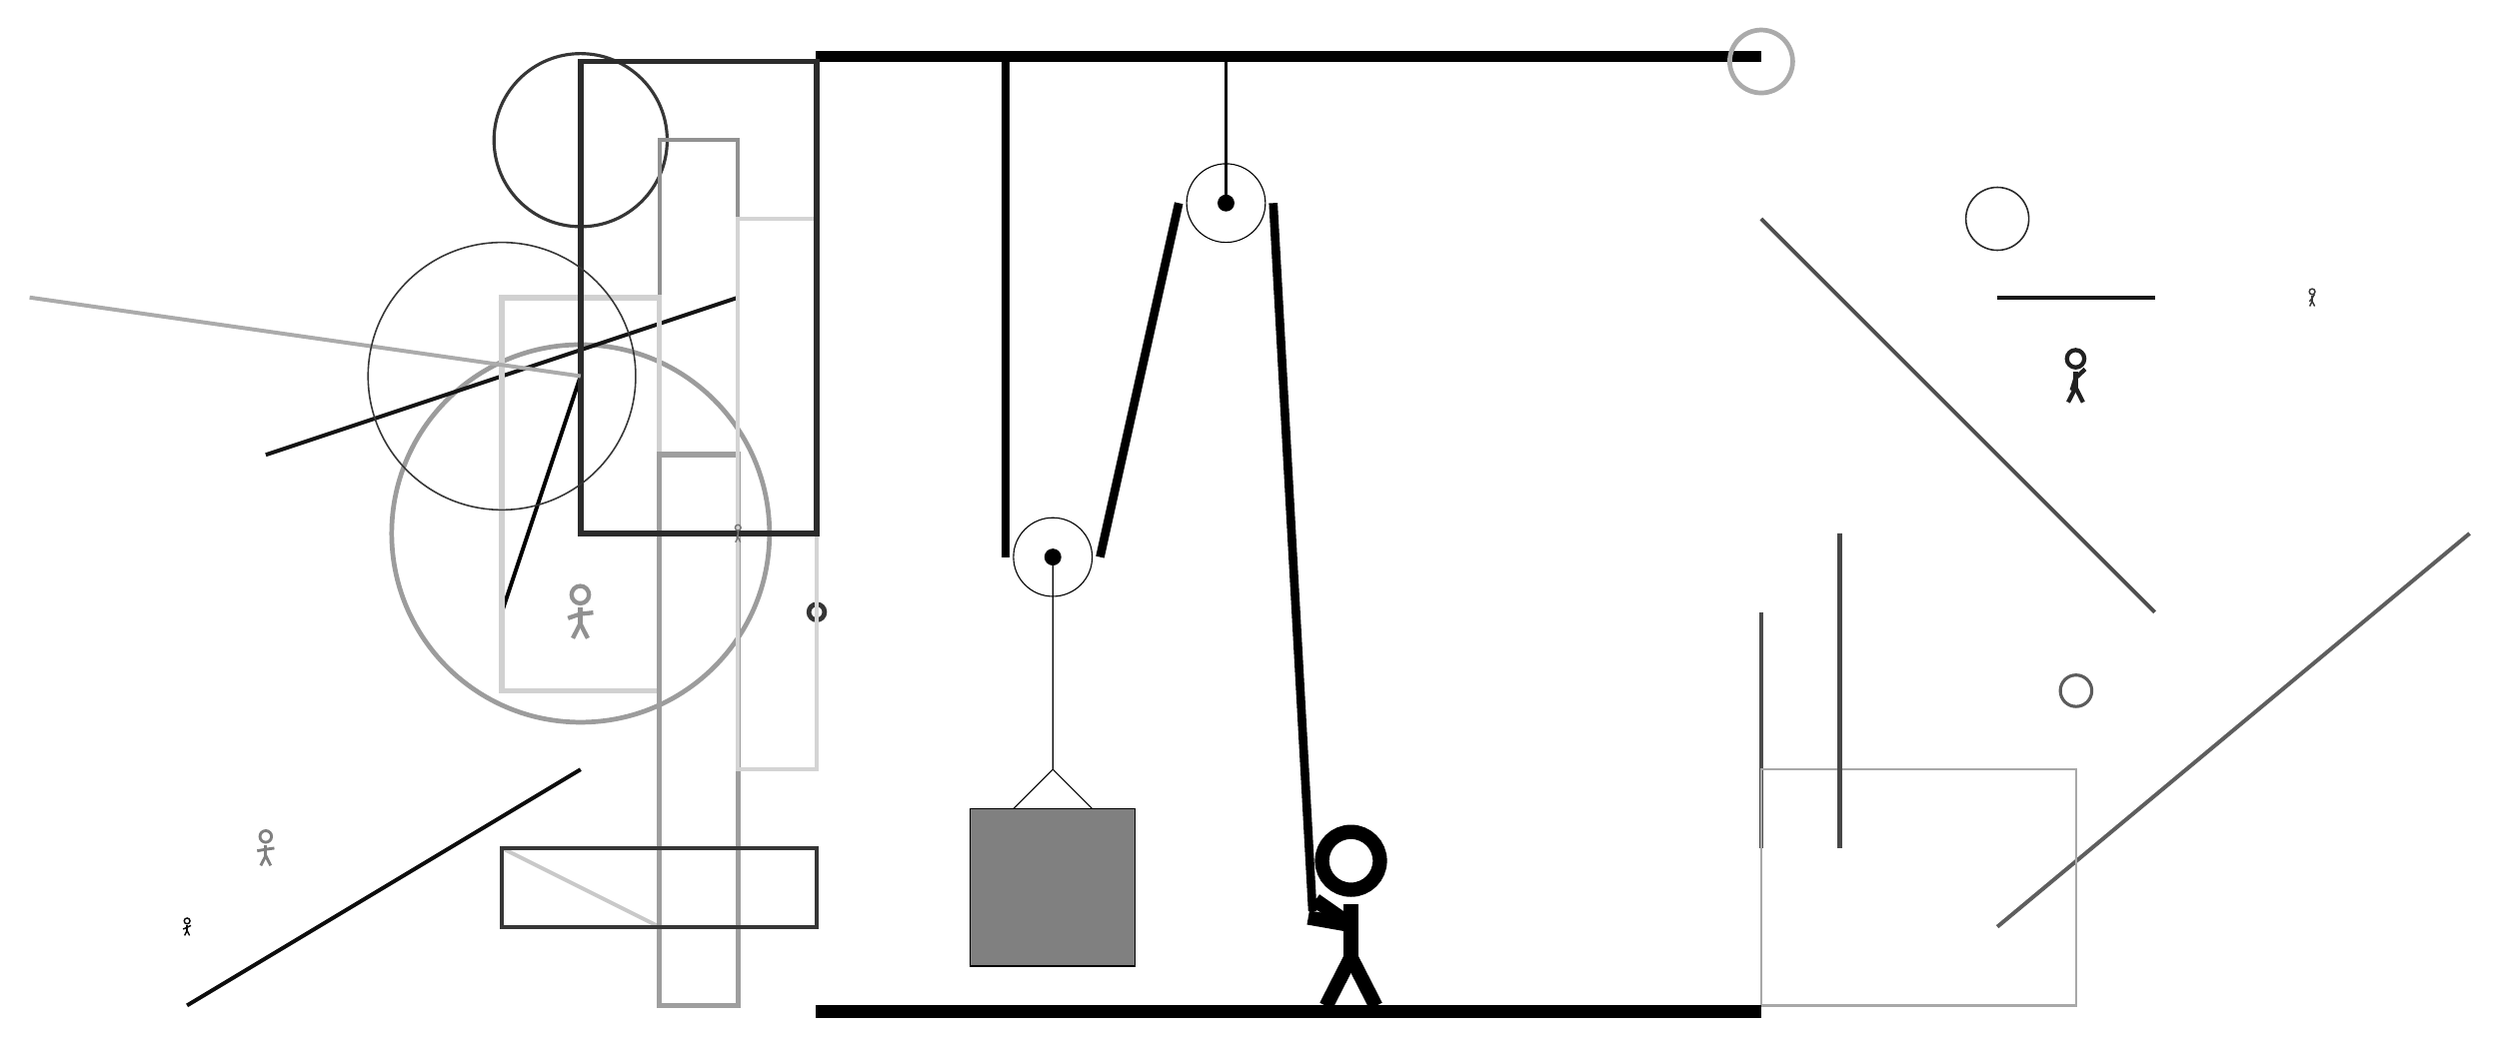
\begin{tikzpicture}
			%%%%% START %%%%%
			
			\draw[fill=black] (-2, 9) rectangle (10, 9.125);
			
			\draw (3.2, 7.2) circle (0.5);
			\draw[fill=black] (3.2, 7.2) circle (0.1);
			\draw[thick] (3.2, 7.2) -- (3.2, 9);
			
			\draw (1, 2.7) circle (0.5);
			\draw[fill=black] (1, 2.7) circle (0.1);
			
			\draw (1, 2.7) -- (1, 0) -- (0.5, -0.5);
			\draw (1, 0) -- (1.5, -0.5);
			\draw[fill=black!50] (-0.05, -0.5) rectangle (2.05, -2.5);
			
			\draw [line width=0.6mm, color=black!39](-5, 3) circle (2.4);
			
			\draw[line width=0.5mm, color=black!70](10, 2) -- (10, -1);
			\draw[line width=0.5mm, color=black!69](15, 2) -- (10, 7);
			\draw [line width=0.4mm, color=black!79](-5, 8) circle (1.1);
			\draw[line width=0.5mm, color=black!63](13, -2) -- (19, 3);
			\node[line width=0.5mm, color=black!78] at (17, 6) {\Strichmaxerl[1][52][59]};
			\draw[line width=0.5mm, color=black!43] (-3, -1) rectangle (-4, 8);
			\draw[line width=0.3mm, color=black!34] (10, -3) rectangle (14, 0);
			\draw[line width=0.5mm, color=black!92](-3, 6) -- (-9, 4);
			\draw[line width=0.5mm, color=black!21](-4, -2) -- (-6, -1);
			\draw [line width=0.6mm, color=black!79](-2, 2) circle (0.1);
			\draw[line width=0.5mm, color=black!100](-5, 5) -- (-6, 2);
			\draw[line width=0.7mm, color=black!18] (-4, 6) rectangle (-6, 1);
			
			\draw [line width=0.2mm, color=black!90](-10, 8) circle (0.0);
			\draw[line width=0.7mm, color=black!38] (-4, -3) rectangle (-3, 4);
			\draw[line width=0.5mm, color=black!17] (-3, 0) rectangle (-2, 7);
			
			\node[line width=0.5mm, color=black!50] at (-9, -1) {\Strichmaxerl[2][10][8]};
			
			\draw[line width=0.6mm, color=black!72] (11, 3) rectangle (11, -1);
			\draw [line width=0.4mm, color=black!64](14, 1) circle (0.2);
			\draw[line width=0.7mm, color=black!83] (-2, 3) rectangle (-5, 9);
			\draw[line width=0.5mm, color=black!79] (-2, -1) rectangle (-6, -2);
			\draw [line width=0.6mm, color=black!33](10, 9) circle (0.4);
			
			\draw [line width=0.2mm, color=black!84](13, 7) circle (0.4);
			\node[line width=0.5mm, color=black!87] at (14, 5) {\Strichmaxerl[3][73][43]};
			\draw[line width=0.5mm, color=black!33](-5, 5) -- (-12, 6);
			
			\node[line width=0.7mm, color=black!54] at (-3, 3) {\Strichmaxerl[1][74][88]};
			
			\node[line width=0.6mm, color=black!43] at (-5, 2) {\Strichmaxerl[3][19][6]};
			\draw [line width=0.2mm, color=black!79](-6, 5) circle (1.7);
			\draw[line width=0.5mm, color=black!95](-5, 0) -- (-10, -3);
			\draw[line width=0.5mm, color=black!90](13, 6) -- (15, 6);
			\node[line width=0.3mm, color=black!96] at (-10, -2) {\Strichmaxerl[1][24][26]};
			
			
			\draw[line width=1.1mm] (0.4, 9) -- (0.4, 2.7);
			\centerarc[line width=1.1mm](1, 2.7)(180:360:0.6);
			\draw[line width=1.1mm](1.6, 2.7) -- (2.6, 7.2);
			\centerarc[line width=1.1mm](3.2, 7.2)(0:180:0.6);
			\draw[line width=1.1mm](3.8, 7.2) -- (4.3, -1.8);
			
			\node at (4.7, -1.9) {\Strichmaxerl[10][-35][170]};
			
			\draw[fill=black] (-2, -3) rectangle (10, -3.15);
			
			%%%%% END %%%%%
		\end{tikzpicture}
	\end{figure}	
\end{document}